\chapter{Related Work}\label{related}
\section{Projekte mit automatisierten Lege-Robotern}
Die Automatisierung der Baubranche hat neben Faktoren wie Geschwindigkeit, Effizienz und Kostenreduzierung auch den Vorteil Bauprojekte an Orten zu realisieren, die für Menschen ungeeignet sind~\cite{Petersen2012}.
Dafür wurde unter anderem das Projekt \textit{TERMES} von Kirstin Petersen et al.\ konzipiert, mit welchem das Team, angelehnt an dem Verhalten von Termiten, einen Schwarm bodengebundener Roboter koordiniert, die als Einheit Strukturen errichten~\cite{Petersen2012}.
Darüber hinaus stellen Kirstin Petersen et al.\ in einer anderen Veröffentlichung eine umfangreiche Übersicht von weiteren Projekten aus dem Bereich \textit{Collective Robotic Construction} vor~\cite{Petersen2019}.
Doch nicht nur vollautomatische Roboterschwärme haben das Ziel die Baubranche zu verändern.
Es gibt bereits etablierte Firmen, die semi-automatische Roboteranlagen zur Unterstützung der Arbeiter vor Ort anbieten und damit erfolgreich die Bauzeit reduzieren können.
Dazu zählt zum Beispiel \textit{Hadrian X} der Firma FBR:\ ein mobiler, bodengebundener Kran der in der Lage ist, ausgehend von einem CAD Modell, ein bis zu drei Stockwerke hohes Gebäude aufzuschichten~\cite{HadrianX}.
Ein weiteres Beispiel stellt \textit{SAM100} dar, ein mobiler, Ziegelstein legender Roboter der Firma \textit{Construction Robotics}~\cite{SAM}.
Dieser kann sich sogar erhöht auf einem Gerüst bewegen und damit in jedem Stockwerk zum Einsatz kommen.

\section{Planungsvorgehen}\label{related:planungsvorgehen}
Grundlage für sämtliche Projekte, in welchen mithilfe von Lege-Robotern automatisiert Gebäude beziehungsweise Gebilde mit Formsteinen errichtet werden, ist eine vorangehende Planungsphase.
In dieser Planungsphase müssen die notwendigen Informationen zu allen benötigten Bausteinen gesammelt werden, um im Anschluss die Bauphase überhaupt zu ermöglichen.
Das sogenannte \textit{Wall Detailing} stellt ein ähnliches Problem wie das \textit{3D Bin Packing Problem} dar und errechnet, ausgehend von einem 3D Modell eines Gebäudes und Informationen zu den gewünschten Mauerwerksverbänden und Bausteinformen, einen möglichen Bauplan für das gesamte Gebäude.
Unter dem \textit{Bin Packing Problem} (im Deutschen als Behälterproblem bekannt) versteht man das möglichst platzsparende Schichten von Objekten in einen oder mehrere limitierte Behälter.
Dies kann sowohl im zwei- als auch im dreidimensionalen Raum geschehen.
Besonders herausfordernd ist das Verteilen unregelmäßig geformter Objekte wie es etwa Xiao Liu et al.\ am Beispiel verschiedener geometrischer Formen oder Qiruyi Zuo et al.\ am Beispiel von Obstkisten zeigen~\cite{Liu2015}~\cite{Zuo2022}.
Während sich in diesem Bereich viel mit unregelmäßig geformten Objekten beschäftigt wird, kann im Falle von Wänden, die mit Bausteinen errichtet werden, eine Einschränkung auf quaderförmige Objekte vorgenommen werden.
Zudem ist das Ziel des \textit{Wall Detailings} nicht eine möglichst gute, sprich eine möglichst lückenlose Lösung zu finden, sondern eine, die sinnvoll aufgeschichtete Wände hervorbringt.
Dabei stellen vor allem Übergänge zwischen mehreren Wandstücken besonders kritische Bereiche dar, für die es vor Ort oft Expertenwissen benötigt.
Zusätzlich muss Mauerwerk in Deutschland und Europa einigen Normen entsprechen. 
Darauf wird in Kapitel~\ref{basics:Mauerwerksbau} näher eingegangen.
Nachfolgend werden aber zunächst einige Veröffentlichungen vorgestellt, die ein ähnliches Ziel wie diese Arbeit verfolgen.

\subsection{Digital Plan of Brickwork Layout for Robotic Bricklaying Technology}\label{related:digital_plan_of_brickwork_layout}
In diesem wissenschaftlichen Papier stellen Usmanov et al.\ ein generelles Vorgehen für das Erstellen eines Ziegel-Legeplans für ein als digitales Modell vorliegendes Gebäude vor~\cite{Usmanov2021}.
Dieses Vorgehen gliedern sie in sechs Schritte:
\begin{figure}[h!]
    \centering
    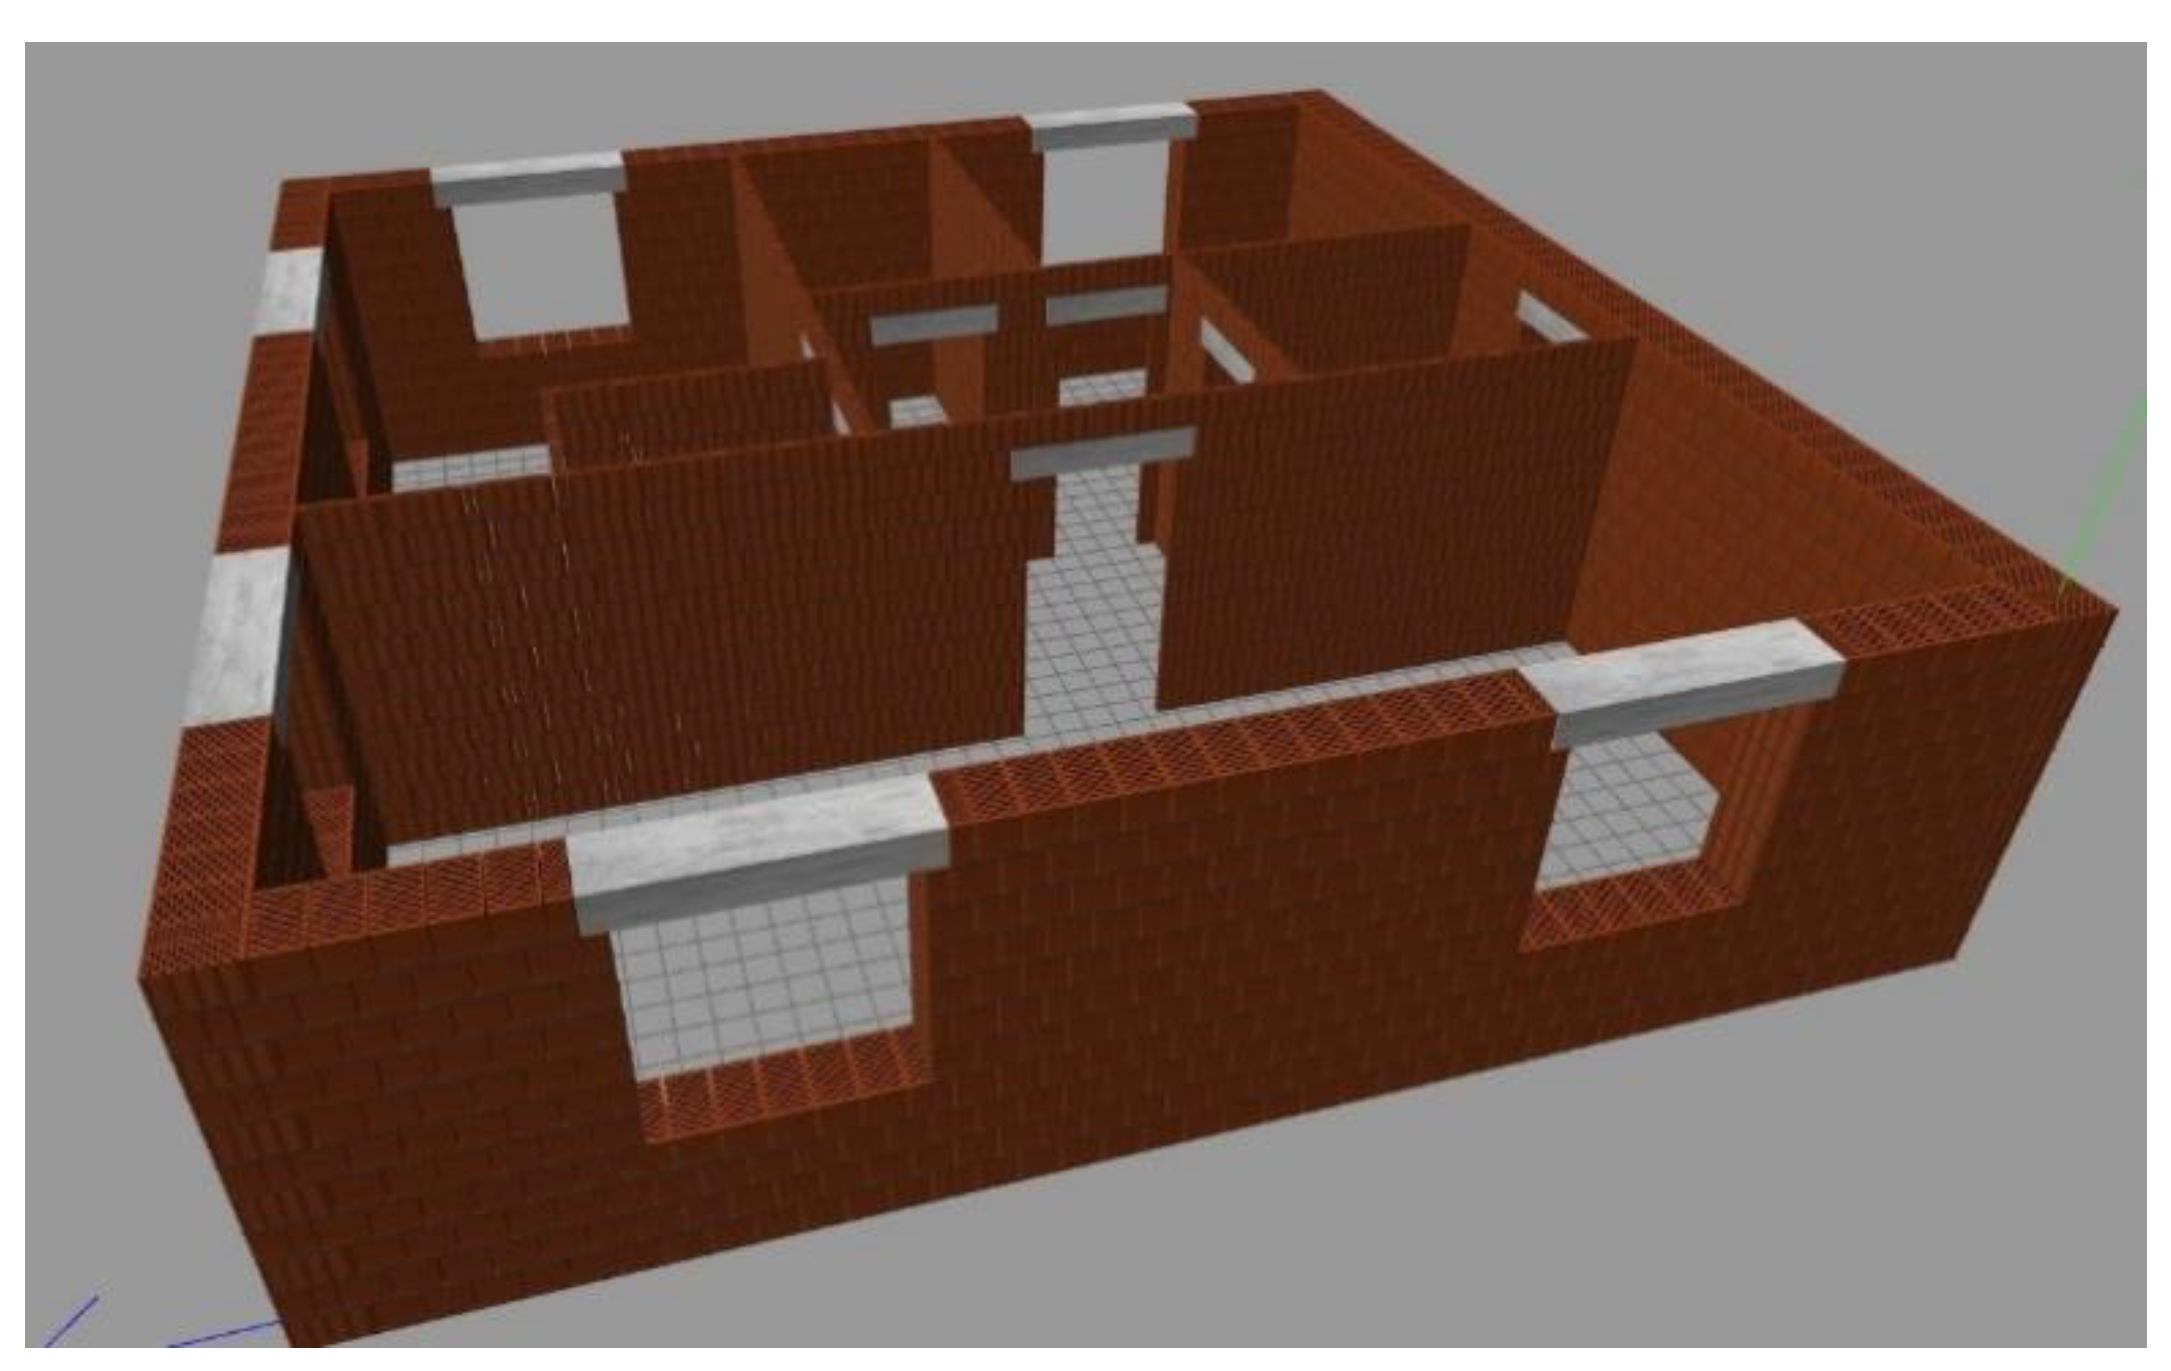
\includegraphics[width=0.5\columnwidth]{fig/sustainability1303905g004.png}
    \caption{Ergebnis des Verfahrens zur Erstellung eines Ziegel-Legeplans nach Usmanov et al.~\cite{Usmanov2021}.}\label{fig:related:usmanov}
\end{figure}
\begin{enumerate}
\item Das vorliegende IFC Modell (siehe~\ref{basics:ifc}) nach Wandelementen durchsuchen und diese in das sogenannte BREP-Format konvertieren.
\item Das Aufteilen des gesamten Modells in Schichten, die der Modulhöhe des verwendeten Ziegelsteinformats entspricht.
\item Verbindungen von getrennt modellierten Wandelementen heraussuchen. 
Dies ist zum Beispiel an Eckstücken der Fall, da dafür oft zwei einzelne Wandelemente modelliert werden, welche in einem Winkel zueinander stehen und sich berühren. 
Für die nachfolgenden Schritte sind diese Verbindungen relevante Informationen.
\item Mit den Informationen der vorangegangenen Schritte können nun für jede Schicht kritische Bereiche identifiziert werden, an welchen später ein komplexer Legevorgang von Ziegeln vonnöten ist.
\item Nun werden zunächst die kritischen Bereiche anhand einer vorher definierten Legeanleitung mit teilweise angepassten Ziegelsteinen bestückt und im Anschluss die restlichen Bereiche aller Wände mit dem ausgewählten Standardziegel aufgefüllt. 
In diesem Schritt werden zusätzlich Fenster- und Türstürze über deren Öffnungen in den Wänden gelegt.
\item Dieser Schritt fasst das Anzeigen als 3D Modell und Konvertieren des Resultats in eine nicht konkreter definierte Listenform zusammen. 
Das Ergebnis für das von den Autoren ausgewählte Beispielgebäude ist in Abbildung~\ref{fig:related:usmanov} zu sehen. 
\end{enumerate}

Besonders detailliert ist ihr Ansatz für das Finden von besagten kritischen Teilbereichen einer Wand mithilfe mathematischer Gleichungen, die alle Wände zueinander in Beziehung stellen.
Diese Teilbereiche sind Wandecken, T-Kreuzungen (wie etwa der Übergang einer Innenwand an eine Außenwand) und Öffnungen innerhalb einer Wand und sind ebenfalls in Kapitel~\ref{scenarios:scenario2} dieser Arbeit als Fallbeispiel aufgeführt.
Anhand der von ihnen zusammengetragenen Informationen konnten die Autoren erfolgreich die bestmögliche Platzierung von vier Roboterarmen errechnen, die den schnellstmöglichen Bau des Gebäudes ermöglichen.
Dennoch werden zum Schluss noch einige Einschränkungen ihres Verfahrens angesprochen.
Vor allem die Beschränkung auf 90\textdegree{} Ecken und das Gebunden sein an einen einzigen Standardziegel werden als besonders restriktiv wahrgenommen.
Außerdem fehlt die Unterstützung anderer Mauerwerksverbände.

\subsection{Optimal brick layout of masonry walls based on intelligent evolutionary algorithm and building information modeling}
Xu Chengran et al.\ haben in dieser Veröffentlichung verschiedene Optimierungsansätze aus dem Bereich des 2D Packaging Problems getestet~\cite{Xu2021}.
Konkret wurden drei Algorithmen verwendet: Differential Evolution, Particle Swarm Optimization und Neighbourhood Field Optimization.
Außerdem wird ein dreiphasiges Vorgehen vorgeschlagen: \textit{Data collection}, \textit{Brick layout} und \textit{Data Output}.
Dieses Vorgehen ähnelt dem von Usmanov et al.\ und eignet sich ebenfalls für das Konzept dieser Arbeit, da zuerst alle relevanten geometrischen Daten aus dem 3D Modell gesammelt werden müssen, bevor das eigentliche \textit{Wall Detailing} stattfinden kann.
Nach dem Optimieren der Bausteinkonfiguration muss das Ergebnis ebenfalls in ein Format gebracht werden, das für die nachfolgenden Schritte verwendet und eventuell auch dem Nutzer angezeigt werden kann.
Dennoch werden auch in dieser Veröffentlichung lediglich zwei verschiedene Mauerwerksverbände betrachtet, die zwar von den Optimierungsalgorithmen umgesetzt werden konnten, aber nur an geraden Wandstücken getestet wurden.
Das Anwenden der Lösungsalgorithmen auf Eck- und Kreuzungsbereiche stellt einen sinnvolleren Anwendungsfall dar, als damit das \textit{Wall Detailing} gerader Wandabschnitte zu lösen.
Letzteres kann, was mit dieser Arbeit gezeigt wird, ebenso iterativ berechnet werden.
Dadurch werden potenzielle Fehler der Optimierungsalgorithmen verhindert.
Das Lösen der kritischen Bereiche entspricht hingegen eher einem Problem, das mit \glqq{}intelligenten\grqq{} Optimierungsverfahren bewältigt werden kann. 

\subsection{Automated Brick Pattern Generator for Robotic Assembly using Machine Learning and Images}
Bárbara Andrade Zandavali et al.\ untersuchen in ihrem Paper wie gut sich Machine Learning Algorithmen dazu eignen, anhand von Bildern Pläne für konkretes Mauerwerk zu erzeugen~\cite{Zandavali2019}.
Ein Kernaspekt dabei war das Anwenden verschiedener Mauerwerksverbände auf arbiträre Vielecke, welche die Form eines Wandabschnitts beschreiben.
\begin{figure}[ht!]
    \centering
    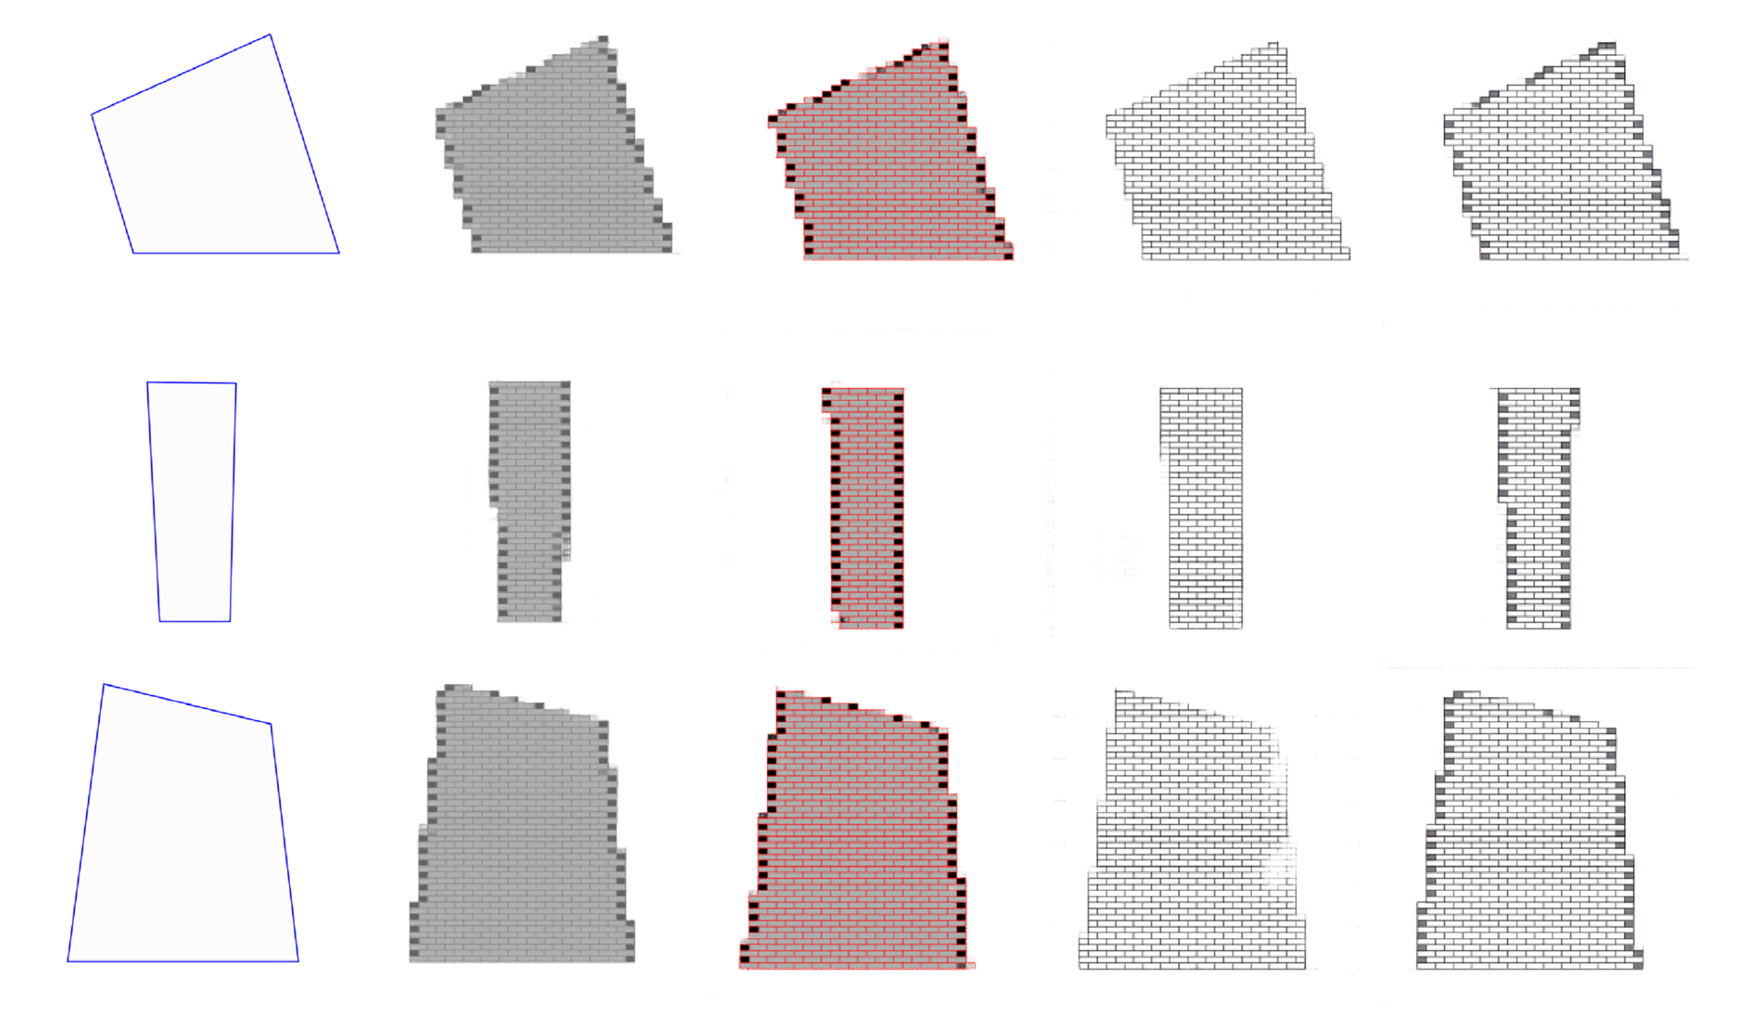
\includegraphics[width=0.8\columnwidth]{fig/ecaadesigradi2019_605.png}
    \caption{Eingaben und Ergebnisse des \textit{Brick Pattern Generator} nach Bárbara Andrade Zandavali et al.~\cite{Zandavali2019}.}\label{fig:related:Zandavali2019}
\end{figure}
In Abbildung~\ref{fig:related:Zandavali2019} sind verschiedene Eingabeformen (linke Spalte) und deren Ergebnisse in vier verschiedenen Ausgabearten zu sehen.
Da es sich sowohl bei dem Eingabe- als auch bei dem Ausgabeformat um Bilder handelt, musste im Anschluss zunächst untersucht werden, wie gut sich die verschiedenen Ergebnisarten dazu eignen daraus tatsächliches Mauerwerk zu interpretieren.
Zusammenfassend konnten die Autoren berichten, dass das Vorgehen teilweise zu fragwürdigen Resultaten geführt hat, welches sich aber mit Sicherheit durch Anpassungen von Parametern des Algorithmus verbessern lässt.
Dennoch ist der Anwendungsfall gerader Wandabschnitte schlecht gewählt, da sich dieselben Ergebnisse auch durch \glqq{}Ausstanzen\grqq{} der Vielecke aus einer zuvor mit Bausteinen aufgefüllten, rechteckigen Wand erreichen lassen.
Das Anwenden intelligenter Mechanismen wie Machine Learning zum automatischen Lösen der kritischen Eck- und Kreuzungsbereiche zwischen mehreren Wandstücken kann sich allerdings, wie bereits erwähnt, durchaus als nützlich erweisen.

\subsection{Parametric Blockwall-Assembly Algorithms for the Automated Generation of Virtual Wall Mockups Using BIM}
Tarek Zaki et al.\ beschreiben in dieser Veröffentlichung ein Vorgehen, das es ermöglicht die Werkstatt- und Montageplanung für ein Bauprojekt, das in einer BIM-fähigen Umgebung geplant wird, direkt innerhalb derselben Umgebung durchführen zu können~\cite{Zaki2017}.
Dies wurde bisher von Hand als zusätzliches sogenanntes \textit{Level of Detail} (LOD) berechnet und im Anschluss wieder in das Projekt integriert.
Das angestrebte LOD ist eine Art Mockup und siedelt sich einen Schritt vor dem letzten LOD, dem Baubestandsplan, an.
Baubestandspläne stellen eine exakte Repräsentation der zu bauenden Elemente dar.
Das Ziel der Veröffentlichung ist, dieses LOD direkt in der BIM Umgebung zu berechnen und anzuzeigen, da darin die dafür notwendigen Informationen ohnehin vorhanden sind.
Insgesamt soll dies eine genauere Materialanalyse und Kostenplanung ermöglichen.
Da es sich aber \glqq{}nur\grqq{} um ein Mockup handelt, werden zum Beispiel Eckbereiche nicht berücksichtigt, sondern durch sich überlappende Wandstücke und Bausteine realisiert.
Dafür kann jedoch ein beliebiges Basismodul vorgegeben werden, das nach Erstellen des Mockups bereits offensichtliche Fehler sichtbar macht.
So überschneidet sich etwa ein deplatziertes Fenster mit dem Mauerwerk, wenn sich dieses nicht auf dem durch das Grundmodul vorgegebene Raster befindet.
Dennoch soll das Ergebnis dieser Arbeit im Gegensatz dazu ein konkreter Bauplanentwurf sein, der direkt in die Realität überführt werden kann; sei es von Robotern oder Menschen oder einer Kombination aus beiden.